\chapter{Results}
\label{sec:results}

In the following sections, we discuss all the outcomes brought by data analysis, which supports the research questions defined in our study. In the first subsection (Section \ref{sec:overalAgreement}) we present the agreement considering all members who participate in our study, we summarize the evaluations and calculate the agreement using Fleiss Kappa measure. In further sections, we will refine the results from Section \ref{sec:overalAgreement} presenting the agreement among participants by considering different factors related to them, such as their origin (Section \ref{sec:originAgreement}) and experience (Section \ref{sec:participantExperienceAgreement}). These results help us to answer \textbf{RQ1}. In our study, we do our best to describe and discuss only statistically significant Kappa values by considering a \textit{p-value} < 0.05. Despite it was not possible in some cases.

In Section \ref{sec:effortSpentAnswerTasks} we address the effort spent by participants to accomplish the tasks considering both evaluation modes - with and without decision tree visualization, whose result answers the  \textbf{RQ2}. Finally, the results related to the usefulness of decision tree for decision making, which helps to answer the \textbf{RQ3}, is described in Section \ref{sec:usefulnessDecisionTree}. The results and materials used in our empirical study are available at \hyperlink{https://git.io/Jv6cM}{https://git.io/Jv6cM}.

\section{Overall participants' agreement} \label{sec:overalAgreement}

For the first subsection, we summarize all evaluations provided by participants separated by scenarios, i. e., the scenario with decision tree visualization (\textit{DT}) and without decision tree visualization (\textit{No DT}), as we may see in Table \ref{tbl:overallTableAgreement}. Each row corresponds to the task accomplished by the participants, the column \textit{Code Smell} identifies the type of code smell that was suggested by the task. Each cell, under the columns named \textit{Disagreed} and \textit{Agreed}, represents the sum of evaluations made by participants.

%In both scenarios we can observe that code smells which emphasizes lines of code, like God Class (GC) and Long Method (LM), have the largest difference between who votes 'disagreed' or 'agreed'. It confirms previous studies that such code smells types tend to be more perceived to developers \cite{palomba2014they}, reaching more agreement \cite{hozano2018you} about the occurrence of them in many software codes.
%Otherwise, Refused Bequest has almost the same number of participants that agree and disagree about its occurrence in a given source code. It also confirms the assumptions brought by \cite{hozano2018you}, when the authors empirically demonstrated that such code smell type have a high divergence about its occurrence in source code. 

The inter-rater agreement is calculated using Fleiss Kappa statistical method and the results are showed in Table \ref{tbl:overallKappaValues}, with associated \textit{p-Value} ranged from 0.0388 to 0.2710. The agreement values were calculated considering all tasks from the same group, divided by evaluations made considering the scenario with decision tree (\textit{DT}) and without decision tree (\textit{No DT}). In other words, the agreements were calculated based on each cell of the experiment design illustrated previously in Figure \ref{fig:latinSquare}. 

To classify the agreement strength properly, we interpret what is the degree of agreement of a measured sample based on a scale of categories. These categories were proposed by Landis e Koch \cite{landis1977measurement} and have been adopted by previous works \cite{schumacher2010building,zhang2011code} in order to verify the strength of the Kappa value. The scale of categories is shown in Table \ref{tbl:agreementClassification}. Therefore, we may see that all measures of Table \ref{tbl:overallKappaValues} have a slight agreement strength, regardless of task group or scenario. It confirms the thesis \cite{hozano2018you} that the agreement among developers is commonly low. 

\begin{table*}[ht]
\centering
\begin{tabular}{ll} 
\toprule
Kappa & Agreement Strength~ \\ 
\midrule
\textless{} 0 & Less than chance agreement \\
0.01–0.20~ & Slight agreement~ \\
0.21– 0.40 & Fair agreement \\
0.41–0.60 & Moderate agreement \\
0.61–0.80 & Substantial agreement \\
0.81–0.99 & Almost perfect agreement \\
\bottomrule
\end{tabular}
\caption{Agreement strength categories}
\label{tbl:agreementClassification}
\end{table*}

\begin{table}[ht]
\centering
\begin{tabular}{llccclcc} 
\toprule
 &  & \multicolumn{1}{l}{} & \multicolumn{2}{c}{DT scenario} & \multicolumn{1}{c}{} & \multicolumn{2}{c}{No DT scenario} \\ 
\cmidrule{4-5}\cmidrule{7-8}
Group & Task ID & Code Smell & Disagreed & Agreed~ &  & \multicolumn{1}{l}{Disagreed} & \multicolumn{1}{l}{Agreed~} \\ 
\midrule
\multirow{4}{*}{1} & 3 & god class & 1 & 13 &  & 2 & 14 \\
 & 4 & long method & 1 & 13 &  & 0 & 16 \\
 & 11 & long parameter list & 0 & 14 &  & 5 & 11 \\
 & 7 & refused bequest & 5 & 9 &  & 4 & 12 \\ 
\midrule
\multirow{4}{*}{2} & 8 & god class & 2 & 14 &  & 1 & 13 \\
 & 6 & long method & 2 & 14 &  & 3 & 11 \\
 & 12 & long parameter list & 7 & 9 &  & 7 & 7 \\
 & 5 & refused bequest & 8 & 8 &  & 5 & 9 \\
\bottomrule
\end{tabular}
\caption{Overall evaluations}
\label{tbl:overallTableAgreement}
\end{table}

\begin{table}[ht]
\centering
\setlength{\extrarowheight}{0pt}
\addtolength{\extrarowheight}{\aboverulesep}
\addtolength{\extrarowheight}{\belowrulesep}
\setlength{\aboverulesep}{0pt}
\setlength{\belowrulesep}{0pt}
\begin{tabular}{lccl} 
\toprule
 & \multicolumn{1}{l}{Task Group 1} & \multicolumn{1}{l}{Task Group 2} & \multicolumn{1}{c}{{\cellcolor[rgb]{0.753,0.753,0.753}}Avg} \\ 
\midrule
DT & \textbf{0.108 } & \textbf{0.087 } & {\cellcolor[rgb]{0.753,0.753,0.753}}\textbf{0.098}  \\
No DT & 0.041 & 0.058 & {\cellcolor[rgb]{0.753,0.753,0.753}}0.049 \\
\bottomrule
\end{tabular}
\caption{Overall Fleiss Kappa agreement measures}
\label{tbl:overallKappaValues}
\end{table}

\begin{figure}[ht]
\centering
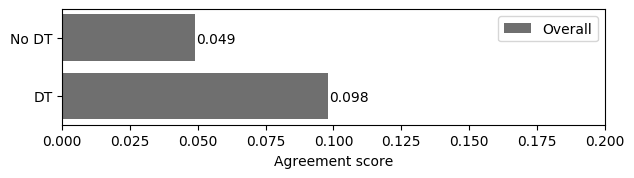
\includegraphics[width=15cm]{figures/overallAgreement.png}
\caption{Average  agreement for all participants.}
\label{fig:averageAgreementOverall}
\end{figure}

The showed Kappa measures tell us that the values from the \textit{DT} scenario (highlighted in bold) overcome the \textit{No DT} scenario in both assessed groups, as well as the average considering the two groups. Hence, the \textit{DT} scenario presented a better agreement among participants compared to the \textit{No DT} scenario. Therefore, it means that the scenario in which the participant obtained insights provided by a visualization from a decision tree model (\textit{DT}) has a relative advantage in terms of agreement. %Therefore, the fact that the scenario "DT" overcomes the scenario "No DT" confirms that the visualization of the rules that describes why certain code snippet was classified as smelly influences the decision making during the evaluation, impacting in the agreement among participants. 

\section{Developer's agreement considering their origin} \label{sec:originAgreement}

During the experiment, we collected information about what is the participant's origin,
if he is from Academy, Industry or both. In the analysis described in the previous section - the overall agreement among participants - we evaluated the inter-rater agreement among all participants responsible for evaluating tasks. At this point, in order to investigate the influence of the origin on the agreement among their evaluations, we split the whole set of participants into subgroups. Due to limitations regarding the number of participants, the only subgroup that deserves a deeper investigation in this subsection is the participants from the academy.

Afterward, we calculate the agreement among the evaluations considering scenarios with and without decision tree visualization. Finally, we compare such subgroup agreement with the overall agreement calculated in section \ref{sec:overalAgreement}. Such comparison allows us to understand whether the origin of the participant plays some role to increase or decrease the agreement among developers when compared to the whole set of participants. 

\subsection{Participants from academy} \label{sec:participantsAcademyAgreement}

In this section, we investigate the agreements reached by participants from the academy, a similar approach as the previous section (Section \ref{sec:overalAgreement}). The Table \ref{tbl:academyKappaValues} shows the Kappa values and the Table \ref{tbl:academyTableEvaluation} clarifies how was distributed the evaluations through tasks and scenarios. The obtained Kappa measures show us that the agreement strength across task groups and scenarios is classified starting from Poor ($Kappa < 0$) up to Slight ($0.01 < Kappa < 0.2$). The Kappa measures highlighted in bold indicate that the agreement in \textit{No DT} scenario overcomes the \textit{DT}scenario in \textit{Task Group 1} whereas the agreement in \textit{DT} scenario overcomes the \textit{No DT} scenario in \textit{Task Group 2}. Despite the average Kappa agreement indicates the \textit{DT} scenario has a better agreement in general, the agreement reached by the \textit{DT} scenario was not better in both tasks group.

\begin{table}[ht]
\centering
\begin{tabular}{llccclcc} 
\toprule
 &  & \multicolumn{1}{l}{} & \multicolumn{2}{c}{DT scenario} & \multicolumn{1}{c}{} & \multicolumn{2}{c}{No DT scenario} \\ 
\cmidrule{4-5}\cmidrule{7-8}
Group & Task ID & Code Smell & Disagreed & Agreed~ &  & \multicolumn{1}{l}{Disagreed} & \multicolumn{1}{l}{Agreed~} \\ 
\midrule
\multirow{4}{*}{1} & 3 & god class & 1 & 7 &  & 1 & 12 \\
 & 4 & long method & 1 & 7 &  & 0 & 13 \\
 & 11 & long parameter list & 0 & 8 &  & 5 & 8 \\
 & 7 & refused bequest & 1 & 7 &  & 3 & 10 \\ 
\midrule
\multirow{4}{*}{2} & 8 & god class & 1 & 12 &  & 1 & 7 \\
 & 6 & long method & 2 & 11 &  & 3 & 5 \\
 & 12 & long parameter list & 6 & 7 &  & 3 & 5 \\
 & 5 & refused bequest & 7 & 6 &  & 2 & 6 \\
\bottomrule
\end{tabular}
\caption{Evaluation table of participants from academy}
\label{tbl:academyTableEvaluation}
\end{table}

\begin{table}[ht]
\centering
\setlength{\extrarowheight}{0pt}
\addtolength{\extrarowheight}{\aboverulesep}
\addtolength{\extrarowheight}{\belowrulesep}
\setlength{\aboverulesep}{0pt}
\setlength{\belowrulesep}{0pt}
\begin{tabular}{lcclc} 
\toprule
 & \multicolumn{1}{l}{Task Group 1} & \multicolumn{1}{l}{Task Group 2} & {\cellcolor[rgb]{0.753,0.753,0.753}}Avg \\ 
\midrule
DT & -0.103 & \textbf{0.112} & {\cellcolor[rgb]{0.753,0.753,0.753}}\textbf{0.004} \\
No DT & \textbf{0.082} & -0.082 & {\cellcolor[rgb]{0.753,0.753,0.753}}0 \\
\bottomrule
\end{tabular}
\caption{Kappa agreement measures of participants from academy}
\label{tbl:academyKappaValues}
\end{table}

\begin{figure}[ht]
\centering
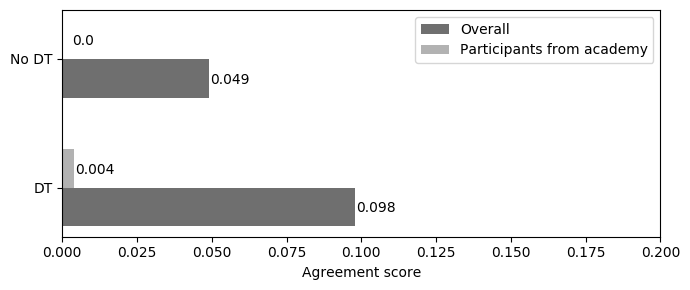
\includegraphics[width=15cm]{figures/overallXacademy.png}
\caption{Average  agreement  comparison: Overall $\times$ participants from academy.}
\label{fig:overallXacademy}
\end{figure}

Figure \ref{fig:overallXacademy} illustrates the average agreement observed in the evaluations done by the participants from the academy and the average agreement from the whole set of participants. In this figure, we use a dark gray bar to represent the overall agreement levels replicated from the average Kappa value of section \ref{sec:overalAgreement}. This plot shows that the average agreement provided by evaluations made by participants from the academy is lower than the overall agreement, both in the \textit{DT} scenario and in the \textit{No DT} scenario. Therefore, the average agreement from participants from academy is fewer compared to the overall.

%Through the analysis of evaluations by task (Table \ref{tbl:academyTableEvaluation}, we can see that the code smells that emphasize the size of lines of code, God Class and Long Method, keep a similar behavior to that seen in the section \ref{sec:overalAgreement}, due to the high difference of participants who voted in "agree" and "disagree".

\section{Agreements by experience} \label{sec:participantExperienceAgreement}

Previously we investigate the inter-rater agreement based on participants’ origin. In this turn, we investigate the agreements taking into account the participants’ experience. In this way, we analyze the agreement among the more experienced participants in three different profiles: code smell detection, Java programming and development.

During the experiment execution, the developer rated his experience by choosing one of five options: "I do not have any experience", "Very low", "Low", "High" and "Very high".  So the experience of each developer is defined by the self-assigned ratings reported by him, so we consider an experienced developer the one who have experience rating above "High". Due to the constraints regarding the number of participants, we also include participants self-rated "Low", it contributed to becoming the results more statistically significant. 

\subsection{Experienced participants on code smell detection} \label{sec:participantsCodeSmellDetecAgreement}    
In this section, we extract a subset of participants who are experienced in code smell detection, putting side by side the agreements obtained by the \textit{DT} scenario and the  \textit{No DT} scenario. 

\begin{table}[ht]
\centering
\begin{tabular}{llccclcc} 
\toprule
 &  & \multicolumn{1}{l}{} & \multicolumn{2}{c}{DT scenario} & \multicolumn{1}{c}{} & \multicolumn{2}{c}{No DT scenario} \\ 
\cmidrule{4-5}\cmidrule{7-8}
Group & Task ID & Code Smell & Disagreed & Agreed~ &  & \multicolumn{1}{l}{Disagreed} & \multicolumn{1}{l}{Agreed~} \\ 
\midrule
\multirow{4}{*}{1} & 3 & god class & 0 & 9 &  & 2 & 7 \\
 & 4 & long method & 0 & 9 &  & 0 & 9 \\
 & 11 & long parameter list & 0 & 9 &  & 2 & 7 \\
 & 7 & refused bequest & 4 & 5 &  & 2 & 7 \\ 
\midrule
\multirow{4}{*}{2} & 8 & god class & 1 & 8 &  & 0 & 9 \\
 & 6 & long method & 1 & 8 &  & 2 & 7 \\
 & 12 & long parameter list & 2 & 7 &  & 6 & 3 \\
 & 5 & refused bequest & 3 & 6 &  & 3 & 6 \\
\bottomrule
\end{tabular}
\caption{Evaluation table of experienced participants on code smell detection}
\label{tbl:codeSmellDetectionTableEvaluation}
\end{table}

\begin{table}[ht]
\centering
\setlength{\extrarowheight}{0pt}
\addtolength{\extrarowheight}{\aboverulesep}
\addtolength{\extrarowheight}{\belowrulesep}
\setlength{\aboverulesep}{0pt}
\setlength{\belowrulesep}{0pt}
\begin{tabular}{lccl} 
\toprule
 & \multicolumn{1}{l}{Task Group 1} & \multicolumn{1}{l}{Task Group 2} & {\cellcolor[rgb]{0.753,0.753,0.753}}Avg \\ 
\midrule
DT & \textbf{0.299} & -0.064 & {\cellcolor[rgb]{0.753,0.753,0.753}}\textbf{0.116} \\
No DT & -0.050 & \textbf{0.183} & {\cellcolor[rgb]{0.753,0.753,0.753}}0.066 \\
\bottomrule
\end{tabular}
\caption{Kappa measure of experienced participants on code smell detection}
\label{tbl:codeSmellDetectionKappaValues}
\end{table}

\begin{figure}[ht]
\centering
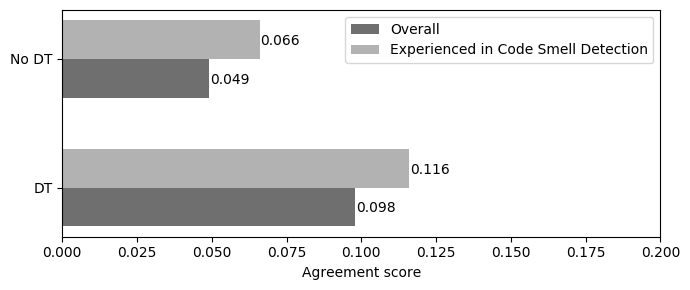
\includegraphics[width=15cm]{figures/overallXcodeSmellIdentification.png}
\caption{Average agreement comparison: Overall $\times$ Experienced participants in code smell detection}
\label{fig:overallxcodeSmellDetection}
\end{figure}

The Table \ref{tbl:codeSmellDetectionTableEvaluation} shows the total of assignments divided by scenario and group of tasks, the Table \ref{tbl:codeSmellDetectionKappaValues} shows the comparison of inter-rater kappa measure among  \textit{DT} scenario and  \textit{No DT} scenario and the Figure \ref{fig:overallxcodeSmellDetection} compares the average agreement that was performed by experienced developers on code smell detection in contrast to the average agreement performed by overall participants. 
%For developers with such type of skill, the tasks with long methods smells (tasks 4 and 6) have three of four evaluations that were unanimous for both scenarios, followed by god class with 2 unanimous evaluations. In fact, it confirms previous sections where tasks which code smell type is based on size performed better in terms of agreement. 

In the Table \ref{tbl:codeSmellDetectionKappaValues}, we can see that the task evaluations carried out by a decision tree visualization (\textit{DT}) have a better agreement on average than the evaluations done without decision tree rules (\textit{No DT}), even though the agreement in \textit{No DT} overcomes the \textit{DT} in Task Group 2. Thus, despite the average of Kappa agreement indicates the \textit{DT} scenario have a better agreement in general, it is not better considering both task group individually.

Comparing the agreement computed through the average of Fleiss Kappa measure with the overall agreement, as shown in Figure \ref{fig:overallxcodeSmellDetection}, the average of agreement from experienced developers on code smell detection performed better than the overall participants. Such result indicates that the expertise of such type of participant in detecting code smells in several software projects brings some uniformity of evaluations, as both scenarios of agreement from experienced developers overcome the overall agreement. Moreover, we may infer that the rules from the decision tree were an important factor for increasing the agreement among developers, thus it may help for accurate reasoning about the smelliness or absence of smell during its detection. 

\subsection{Experienced participants on Java language} \label{sec:participantsJavaAgreement}    

In this section we analyze how the experienced participants on Java language agree in code smell detection, computing the Kappa agreements obtained by \textit{DT} scenario and \textit{No DT} scenario.

Table \ref{tbl:JavaLanguageKappaValues} shows the Kappa agreement values and Table \ref{tbl:javaLanguageTableEvaluation} shows a detailed view of the distribution of evaluations across tasks and scenarios. Differently of previous participant profiles, the obtained Kappa measures indicate that the agreement ranges from 0.018 up to 0.233, i. e., the table indicates that the agreement strength ranges from \textit{slight agreement} up to \textit{fair}. The Kappa measures highlighted in bold indicate that the agreement in \textit{No DT} scenario overcomes the \textit{DT} scenario in Task Group 2 whereas the agreement in \textit{DT} scenario overcomes the \textit{No DT} scenario in Task Group 1. The average agreement considering both tasks group indicates that \textit{No DT} scenario has, in general, a better agreement than the \textit{DT} scenario. 

\begin{table}[ht]
\centering
\begin{tabular}{llccclcc} 
\toprule
 &  & \multicolumn{1}{l}{} & \multicolumn{2}{c}{DT scenario} & \multicolumn{1}{c}{} & \multicolumn{2}{c}{No DT scenario} \\ 
\cmidrule{4-5}\cmidrule{7-8}
Group & Task ID & Code Smell & Disagreed & Agreed~ &  & \multicolumn{1}{l}{Disagreed} & \multicolumn{1}{l}{Agreed~} \\ 
\midrule
\multirow{4}{*}{1} & 3 & god class & 0 & 10 &  & 2 & 10 \\
 & 4 & long method & 1 & 9 &  & 0 & 12 \\
 & 11 & long parameter list & 0 & 10 &  & 3 & 9 \\
 & 7 & refused bequest & 4 & 6 &  & 4 & 8 \\ 
\midrule
\multirow{4}{*}{2} & 8 & god class & 1 & 11 &  & 0 & 10 \\
 & 6 & long method & 1 & 11 &  & 2 & 8 \\
 & 12 & long parameter list & 4 & 8 &  & 7 & 3 \\
 & 5 & refused bequest & 5 & 7 &  & 3 & 7 \\
\bottomrule
\end{tabular}
\caption{Evaluation table of experienced developers on Java language}
\label{tbl:javaLanguageTableEvaluation}
\end{table}

\begin{table}[ht]
\centering
\setlength{\extrarowheight}{0pt}
\addtolength{\extrarowheight}{\aboverulesep}
\addtolength{\extrarowheight}{\belowrulesep}
\setlength{\aboverulesep}{0pt}
\setlength{\belowrulesep}{0pt}
\begin{tabular}{lccl} 
\toprule
 & \multicolumn{1}{l}{Task Group 1} & \multicolumn{1}{l}{Task Group 2} & {\cellcolor[rgb]{0.753,0.753,0.753}}\textbf{Avg} \\ 
\midrule
DT & \textbf{0.162} & 0.046 & {\cellcolor[rgb]{0.753,0.753,0.753}}0.104 \\
No DT & 0.018 & \textbf{0.233} & {\cellcolor[rgb]{0.753,0.753,0.753}}\textbf{0.125} \\
\bottomrule
\end{tabular}
\caption{Kappa measure of experienced Java language participant}
\label{tbl:JavaLanguageKappaValues}
\end{table}

\begin{figure}[!ht]
\centering
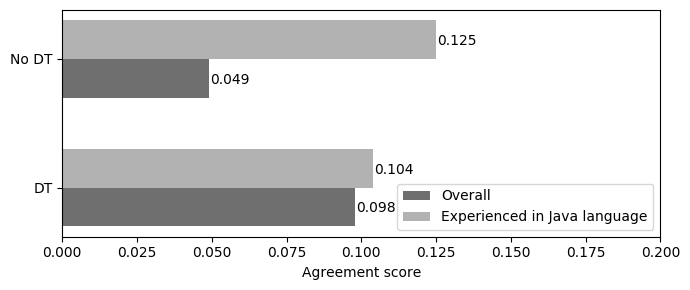
\includegraphics[width=15cm]{figures/overallXjava.png}
\caption{Average agreement comparison: Overall $\times$ Experienced in Java Language}
\label{fig:overallxjavaLanguage}
\end{figure}

Comparing the average agreement with the overall agreement, as shown in Figure \ref{fig:overallxjavaLanguage}, the agreement average of experienced Java language developers performed better than the overall participants in both scenarios. But, among experienced participants in Java language, unlike the experienced participants on code smell detection, the \textit{DT} scenario had a lower agreement than the \textit{No DT} scenario. So we may infer that the decision tree didn't have such importance on the agreement, taking into account that, when it was omitted, they reached a better agreement.

\subsection{Experienced participants on development} \label{sec:participantsDevelopmentAgreement}    
Now we investigate how the experienced developers agree in code smell detection, computing the Kappa measures obtained by \textit{DT} scenario and \textit{No DT} scenario.

The Table \ref{tbl:developmentKappaValues} shows the Kappa agreement values and the Table \ref{tbl:developmentTableEvaluation} shows a detailed view of the distribution of evaluations from tasks and scenarios. From the obtained results of the Kappa measure, we observe that the measures for both scenarios keep the low agreement as usual, with an agreement strength classified as slight.
The Kappa measures highlighted in bold indicate that the agreement in \textit{DT} scenario overcomes the \textit{No DT} scenario in Task Group 1 whereas the agreement in \textit{No DT} scenario overcomes the \textit{DT} scenario in Task Group 2. %Although the average of agreement considering both task group indicates that "DT" scenario have a better agreement than "DT" scenario, for each group of tasks . 

\begin{table}[ht]
\centering
\begin{tabular}{llccclcc} 
\toprule
 &  & \multicolumn{1}{l}{} & \multicolumn{2}{c}{DT scenario} & \multicolumn{1}{c}{} & \multicolumn{2}{c}{No DT scenario} \\ 
\cmidrule{4-5}\cmidrule{7-8}
Group & Task ID & Code Smell & Disagreed & Agreed~ &  & \multicolumn{1}{l}{Disagreed} & \multicolumn{1}{l}{Agreed~} \\ 
\midrule
\multirow{4}{*}{1} & 3 & god class & 1 & 13 &  & 2 & 12 \\
 & 4 & long method & 1 & 13 &  & 0 & 14 \\
 & 11 & long parameter list & 0 & 14 &  & 4 & 10 \\
 & 7 & refused bequest & 5 & 9 &  & 3 & 11 \\ 
\midrule
\multirow{4}{*}{2} & 8 & god class & 2 & 12 &  & 1 & 13 \\
 & 6 & long method & 2 & 12 &  & 3 & 11 \\
 & 12 & long parameter list & 5 & 9 &  & 7 & 7 \\
 & 5 & refused bequest & 7 & 7 &  & 5 & 9 \\
\bottomrule
\end{tabular}
\caption{Evaluation table of experienced participants in development}
\label{tbl:developmentTableEvaluation}
\end{table}

\begin{table}[ht]
\centering
\setlength{\extrarowheight}{0pt}
\addtolength{\extrarowheight}{\aboverulesep}
\addtolength{\extrarowheight}{\belowrulesep}
\setlength{\aboverulesep}{0pt}
\setlength{\belowrulesep}{0pt}
\begin{tabular}{lccl} 
\toprule
 & \multicolumn{1}{l}{Task Group 1} & \multicolumn{1}{l}{Task Group 2} & {\cellcolor[rgb]{0.753,0.753,0.753}}Avg \\ 
\midrule
DT & \textbf{0.108} & 0.044 & {\cellcolor[rgb]{0.753,0.753,0.753}}\textbf{0.076} \\
No DT & 0.012 & \textbf{0.058} & {\cellcolor[rgb]{0.753,0.753,0.753}}0.035 \\
\bottomrule
\end{tabular}
\caption{Kappa measure of experienced participants on development}
\label{tbl:developmentKappaValues}
\end{table}

\begin{figure}[ht]
\centering
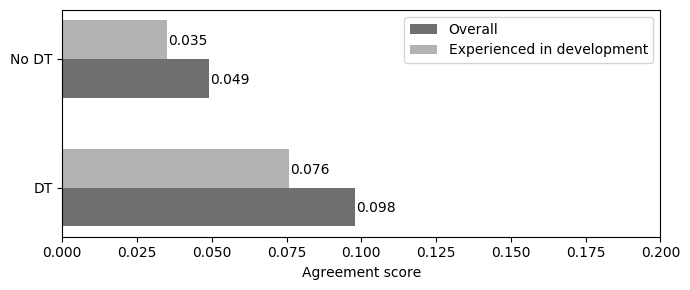
\includegraphics[width=15cm]{figures/overallXdevelopment.png}
\caption{Average agreement comparison: Overall $\times$ Experienced participants in development}
\label{fig:overallxdevelopment}
\end{figure}

Comparing the average agreement of experienced developers with the overall agreement, as shown in Figure \ref{fig:overallxdevelopment}, the agreement of experienced developers performed lower than the overall participants, considering both scenarios. Considering the agreement among experienced participant in development,  the \textit{DT} scenario had a better agreement than the agreement from \textit{No DT} scenario. That result suggest that, for such participant profile, the decision tree visualization have a relative importance on agreement when compared to code inspection without decision tree.


%\subsection{Confidence} \label{sec:participantConfidence}    

% For each question, the respondents were requested to indicate how confident they were that they had provided the correct answer. In Table 8, we provide an overview of the mean confidence per question and representation format. As indicated earlier, confidence was measured on a 5-point scale with 1 = Totally Not Confident and 5 = Very Confident. The bold-face values indicate the representation format for which the confidence is highest. For 12 ofthe 17 questions, the respondents expressed most confidence in their answers when the representation format was a decision table

% \begin{figure}[ht]
% \centering
% 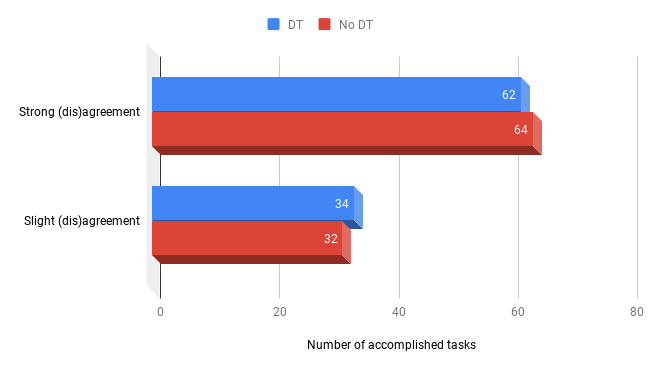
\includegraphics[width=\linewidth]{figures/graph_agreement_confidence.png}
% \caption{Amount of strong and slight dis(agreement)}
% \label{fig:confidenceOfAgreement}
% \end{figure}


\section{The effort spent to answer the tasks} \label{sec:effortSpentAnswerTasks}

For each task of the experiment, we measured the time that the participant spent to accomplish tasks in order to measure effort. Figure \ref{fig:timeSpentAnswerTasks} illustrates boxplots containing the time distribution evolving the two groups of tasks. We dismissed the outliers to adjust the range of analysis from 0 to 16 minutes (y-axis), increasing the comprehension of the graph. 

\begin{figure}[ht]
\centering
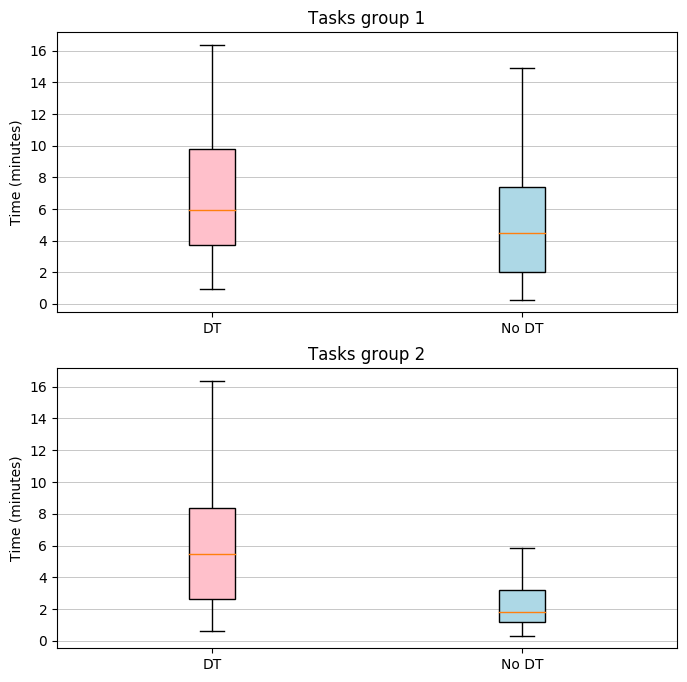
\includegraphics[width=13cm]{figures/graph_boxplot_time_required.png}
\caption{Time spent to answer the tasks}
\label{fig:timeSpentAnswerTasks}
\end{figure}

In the \textit{Tasks group 1}, the time spent to detect code smells aided by decision tree (\textit{DT}) is slightly higher than detecting without it (\textit{No DT}). The slowest time when not aided by the decision tree is faster than the slowest time when detecting code smell aided by a decision tree. The same happens with the quantiles and the minimum.

The \textit{Tasks group 2} presents a higher difference between scenarios \textit{DT} and \textit{No DT} than group 1 regarding the time spent to detect code smells (tasks accomplishment). For this group, the time spent to detect code smells aided by decision tree (\textit{DT}) is considerably higher than detecting without it. The slowest time for \textit{No DT} reaches almost the median of the sample from the opposite scenario \textit{DT}. According to \textit{T-Test}, applied to tasks of Group 2, there is statistically significant evidence (\textit{p-value} = 5.331e-05) that the decision tree visualization doesn't reduce the effort to detect code smells. 

Therefore, for both tasks group, there isn't any evidence that indicates the benefits related to the effort reduction when detecting code smells with a decision tree, i. e., the time spent to detect code smells visualizing the rules provided by a decision tree tends to be equivalent or to overcome the time spent to detect code smells based solely on code inspection. 

\section{The usefulness of decision tree visualization for decision making} \label{sec:usefulnessDecisionTree}

Throughout the participation in the experiment, when faced with the scenario with a decision tree, the participant answered an open question that asked him to inform what insight or contribution the decision tree gave him in order to accomplish the task. We analyzed manually each answer to discover patterns that may indicate the importance of the decision tree for decision making.  From these answers, we apply a coding technique \cite{seaman1999qualitative} to recognize these patterns. 

During the analysis of the open answers, we reject the vague ones. It means that those answers which look like "Helped me so much" or  "It's very helpful" weren't considered. Rather we considered as valid answers those which mention some relevant characteristics like "Number of declarative Lines of Code and Declarative Statements", in this case referring to the metrics within nodes.

Table \ref{tbl:statementsUseful} shows some examples of the statements and the recognized patterns assigned to each, presented in the third column (Detected contribution). Each statement belongs to an answer instance which refers to a task. The ID identifies uniquely the answer given by a participant. The complete list of statements is available in the artifact's repository which accompanies this research\footnote{https://github.com/christianorossini/masterProject}. In total, we categorized 3 contributions that the participants wrote in open question.

\begin{table}
\caption{Example of statements from participants and the detected insight/contribution}
\label{tbl:statementsUseful}
\centering
\setlength{\extrarowheight}{0pt}
\addtolength{\extrarowheight}{\aboverulesep}
\addtolength{\extrarowheight}{\belowrulesep}
\setlength{\aboverulesep}{0pt}
\setlength{\belowrulesep}{0pt}
\begin{tabularx}{\columnwidth}{>{\hsize=0.1\hsize}X>{\hsize=1.2\hsize}X>{\hsize=0.5\hsize}X}
\toprule
\rowcolor[rgb]{0.753,0.753,0.753}  \textbf{ID}      & \textbf{Statement}      & \textbf{Detected contribution}            \\ 
\toprule
491 & \textit{"The lack of cohesion in methods is something I would not be able to compute visually. Thus, the decision tree was handy."} & Information provided by metrics  \\
260 & \textit{"Made the decision more objective (saves time)."} & Facilitates decision  \\
222 & \textit{"Another psychological effect on decision making. A little more confidence in what I had in mind."} & Improved confidence  \\
\bottomrule
\end{tabularx}
\end{table}

\begin{figure}
\centering
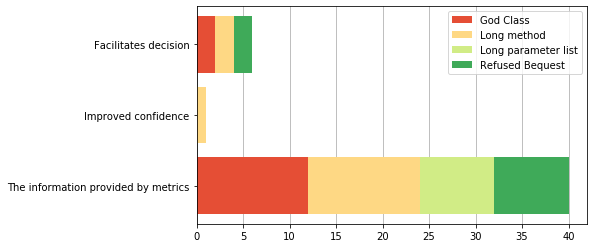
\includegraphics[width=\linewidth]{figures/useful_chart.png}
\caption{The frequency of categorized contributions stated by participants}
\label{fig:usefulchart}
\end{figure}

Figure \ref{fig:usefulchart} presents an overview of number of times these detected contributions was observed in total. From the domain of categorized contributions, the most seen was "The information provided by metrics". So amongst the answers provided by participants, around 85\% stated that the metrics was a important insight to guide their decisions, followed by the fact that the decision tree facilitates the decision of detecting smell (13\%) and the fact that it improves confidence  (2\%). From the last two detected contributions, we can infer that the metric-based rules were a key factor to facilitate smell detection and improve confidence, respectively. Hence, all the categorized contributions involves the rationale of gaining information by metric-based rules. 

When analyzing all the detected contributions in Figure 15 focusing on a type of code smell (that is, a single color), we obtain quantitative information on how many code smells (each one represented by a single decision tree) are present in each detected contribution. For example, the classification models that represent God Class and Long Method are the most evidenced models by those who consider the information provided by metrics as a relevant contribution. Following theses models, on a smaller scale, are the classification models that represent the Long Parameter List and Refused Bequest. Among the available representations of code smell, the Long Parameter List is the only one that is included in all detected contributions.

On the other hand, we also captured the opinions stated by participants who disagree about the usefulness of the decision tree visualization on smell detection, i. e., the participants that stated that certain decision tree didn't contribute to decision making. As previously,  we apply a coding technique \cite{seaman1999qualitative} to recognize patterns obtained from the open question and the Table \ref{tbl:statementsUseless} shows some examples of the statements and the recognized patterns assigned to each one manually. Again, the complete list of statements is available in the artifact's repository\footnote{https://github.com/christianorossini/masterProject}. In total, we categorized 7 different patterns mined from the open answers. 

\begin{table}[t]
\centering
\setlength{\extrarowheight}{0pt}
\addtolength{\extrarowheight}{\aboverulesep}
\addtolength{\extrarowheight}{\belowrulesep}
\setlength{\aboverulesep}{0pt}
\setlength{\belowrulesep}{0pt}
\begin{tabular}{p{1cm}p{10cm}p{3cm}}
\toprule
\rowcolor[rgb]{0.753,0.753,0.753}  \textbf{ID}      & \textbf{Statement example}      & \textbf{Recognized pattern}            \\ 
\toprule
242 & \textit{"The choose by shown decision tree is based only number of lines, this is bad."} & Lack of confidence  \\
192 & \textit{"I was a kind of confuse if number of physical lines are related with only the lines of the parent, used in the child class."} & Confusing rules  \\
224 & \textit{"None. In fact, the tree does not explicitly present "parameters" as a decision criterion."} & Lack of essencial informations  \\
361 & \textit{"couldn't quite understand the "Percent Lack of Cohesion in Methods" metric"} & The metrics understanding  \\
152 & \textit{"Looking at the code was better for me than looking at the tree."} & Code analysis was more effective  \\
121 & \textit{"Not much. The low number of declarative statements says nothing to me about a long parameter list. From my point of view, a method with no declarative statements and few parameters is perfectly possible."} & Useless informations from DT  \\
488 & \textit{"This decision tree gave me the impression of ignoring complexity when deciding on the method's smelliness. Particularly, I disagree with that, because some long methods are not smelly at all. They may be long and, still, easy to read and understand."} & The tree rules mismatch the smell  \\
\bottomrule
\end{tabular}
\caption{Examples of statements from participants who disagrees about the usefulness of decision tree visualization for detecting smells.}
\label{tbl:statementsUseless}

\end{table}

\begin{figure}[ht]
\centering
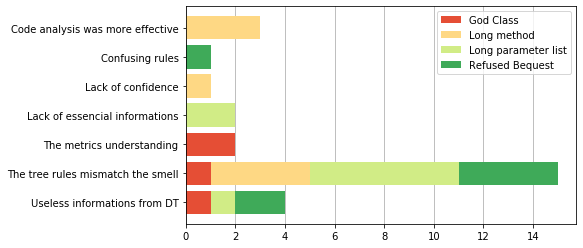
\includegraphics[width=\textwidth]{figures/useless_chart.png}
\caption{The frequency of categorized patterns from statements which considers the decision tree not useful to the context }
\label{fig:uselesschart}
\end{figure}

\begin{figure}[t]
\centering
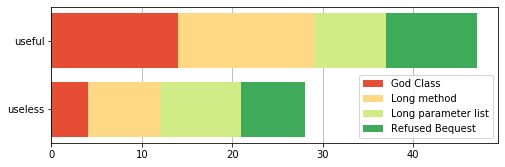
\includegraphics[width=12cm]{figures/useful_useless_total.png}
\caption{The sum of all opinions about the usefulness (contributions) of the classification models (decision tree)}
\label{fig:usefulUselessTotal}
\end{figure}

In the Figure \ref{fig:uselesschart}, we present the number of occurrences of the categorized patterns from the type of statements exemplified in Table \ref{tbl:statementsUseless}.  A large amount of participants states that "The tree rules mismatch the smell", corresponding to 54\% of occurrences, followed by "Useless informations from DT" (14\%), "Code analysis was more effective" (10.71\%), "Lack of essential informations" (7.1\%), "The metrics understanding" (7.1\%), "Lack of confidence" (3.5\%) and "Confusing rules" (3.5\%). Unlike the answers that characterized the classification models as useful for detecting code smells (Figure \ref{fig:usefulchart}), in this case the classification model that represents the God Class has a minor number of occurrences in relation to the other smells. For instance, in the answer categorized as "The tree rules mismatch the smell", the classification model which represents the god class has the lowest number of occurrences. This indicates that the rules contained in the decision tree that represents a god class, basically composed of metrics of size and complexity, proved to be very useful for decision making.  The classification model that represents the Long Parameter List has the majority of opinions that point to the mismatch of the tree rules and the smell that is under evaluation. Besides, it is the only smell representation that is characterized as it lacks essential information for decision making.

In order to summarize the number of opinions categorized as useful or useless, we plot the chart presented in Figure \ref{fig:usefulUselessTotal}. Through the figure we can see, by the number of ocurrences,  that the decision tree (or classification model) which represents the God Class was the most qualified model in terms of the contribution to decision making among the models used, followed by the long method. They have more qualifications defined as 'useful' and less qualifications defined as 'useless'. Therefore, in general, we can conclude that, from the perspective of the participants, there are more answers which indicate that the decision trees gives important insights to the code smell detection process ('Useful' - 63\%) than the opposite ('Useless' - 37\%).










